\section{ Machine learning}

According to Arthur Samuel (qtd. in Geron \cite{geron}) machine learning is a field of study that gives computers the ability to learn without being explicitly programmed.
This ability to learn is the property of various machine learning algorithms.
We will be using terms "machine learning" and "learning" interchangeably. 
In order to learn, these learning algorithms need to be trained on a collection of examples of some phenomenon\cite{burkovml}. 
These collections are called \textbf{datasets} and can be generated artificially or collected in nature.

We can describe a typical ML workflow on an example application.
Let us say that we would like to build a system that can predict a type of animal movement from an accelerometer data.
To train its learning algorithm, also known as a \textbf{model}, we need to expose it to a dataset which would contain accelerometer measurements of different types of movement, such a walking, running, jumping and standing still.
Input to the system could be either raw measurements from all three axis or components extracted from raw measurements such as frequency or amplitude. 
These inputs are also known as \textbf{features}, they are values that describe the phenomenon being observed\cite{burkovml}. 
The output of the system would be a predicted type of movement.
Although we would mark each example of measurement data what type of movement it represents, we would not directly define the relationship between the two.
Instead, we would let the model figure out connection by itself, through the process of training.
The trained model should be general enough so it can correctly predict the type of movement on unseen accelerometer data.

There exists a large variety of different learning algorithms. 
We can broadly categorize them in several ways, one of them depends on how much supervision learning algorithms need in the training process. 
Algorithms like K-nearest neighbours, linear and logistic regression, support vector machines fall into the category of supervised learning algorithms.
Training data that is fed into them includes solutions, also known as \textbf{labels}\cite{geron}.
Described example is an example of a supervised learning problem.

Algorithms like k-Means, Expectation Maximization, Principal Component Analysis fall into the category of unsupervised learning algorithms.
Here training data is unlabeled, algorithms are trying to find similarities in data by itself\cite{geron}.
There exist other categories such as semi-supervised learning which is a combination of previous two and reinforcement learning, where model acts inside environment according to learned policies\cite{geron}.

Neural networks, algorithms inspired by neurons in human brains\cite{geron}\cite{cs231n}, can fall into either of categories. 
They are appropriate for solving complex problems like image classification, speech recognition, and autonomous driving, but they require a large amount of data and computing power for training.
They fall into field of deep learning, which is a sub-field of machine learning.

Training of deep learning algorithms is computationally demanding and is usually done on powerful servers or computers with dedicated graphic processing units to speed up training time.
After a model has been trained, they can feed it data and get prediction in return. 
This process is also known as \textbf{inference}.
The inference is computationally less intensive compared to the training process, so with properly optimized models, we can run inference on personal computers, smartphones, tablets, and even directly in internet browsers.

There are several steps in ML workflow that have to occur in order to get from an idea to a working ML based system as seen on Figure \ref{ml_workflow}.
First problem has to be studied, it has to be understood what are objectives and what approach will be used. Here we decide on rough architecture of the ML model that we will use.
In second step we collect and clean up data.
We should always strive to collect large amount of quality and diverse data that represents real word phenomenon.
Collecting that kind of data can be hard and expensive, but we can use various tools of for producing synthetic data from our original data, thus increasing data size and variety.
Third we train ML model.
We might create something from scratch or use an existing model. 
We can train several different types of models and chose the one that performs the best.
To achieve desired accuracy, steps two and three can be repeated many times.
In step four we deploy our model and monitor its accuracy. We can also use it to collect more data and retrain the model.

\begin{figure}[h]
        \centering
        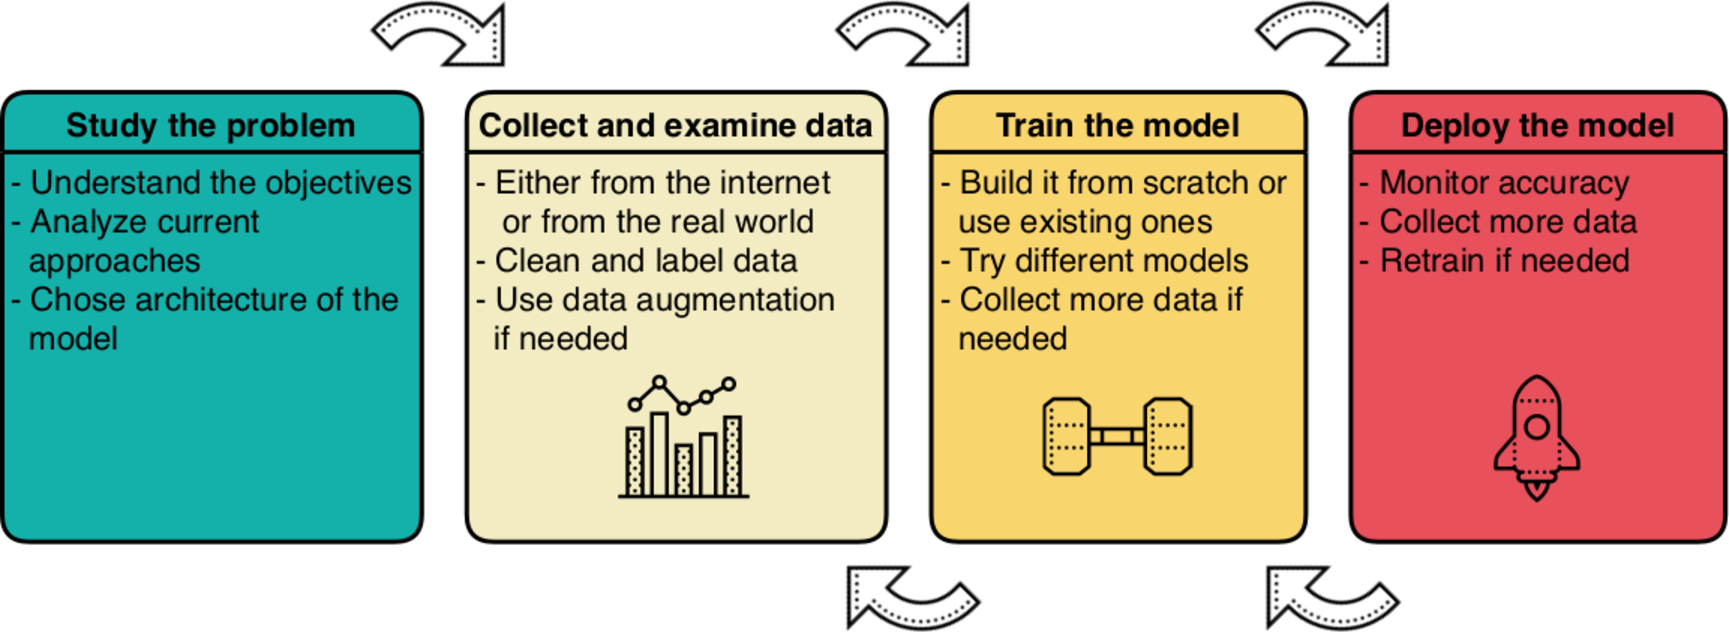
\includegraphics[width=1.0\linewidth]{ml_workflow.pdf} 
        \caption{ Workflow of solving a generic machine learning problem. Icons source: www.icons8.com}
        \label{ml_workflow}
\end{figure}

\subsection{ Machine learning on embedded devices}

Machine learning on embedded devices is an emerging field, which nicely coincides with the Internet of things.
Resources about it are limited, especially when compared to the wast number of resources connected with machine learning on computers or servers.
Most of the information about it can be found in form of scientific papers, blog posts and machine learning framework documentation\cite{hello_edge}\cite{tflite_risc-v}\cite{pete_tiny}.

Running learning algorithms directly on smart devices comes with many benefits.
One of them is reduced power consumption.
In most IoT applications devices send raw sensor data over a wireless network to the server, which processes it either for visualization or for making informed decisions about the system as a whole. 
Wireless communication is one of the more power hungry operations that embedded devices can do, while computation is one of more energy efficient\cite{pete_tiny}.
For example, a Bluetooth communication might use up to 100 milliwatts, while MobileNetV2 image classification network running 1 inference per second would use up to 110 microwatts\cite{pete_tiny}
As deployed devices are usually battery powered, it is important to keep any wireless communication to a minimum, minimizing the amount of data that we send is paramount.
Instead of sending everything we capture, is much more efficient to process raw data on the devices and only send results.

Another benefit of using ML on embedded devices is decreased time between event and action.
If the devices can extract high-level information from raw data, they can act on it immediately, instead of sending it to the cloud and waiting for a response. 
Getting a result now takes milliseconds, instead of seconds.

Such benefits do come with some drawbacks.
Embedded devices are a more resource constrained environment when compared to personal computers or servers.
Because of limited processing power, it is not feasible to train ML models directly on microcontrollers.
Also is not feasible to do online learning with microcontrollers, meaning that they would learn while being deployed.
Models also need to be small enough to fit on a device. 
Most general purpose microcontrollers only offer several hundred kilobytes of flash, up to 2 megabytes.
For comparison, MobileNet v1 image classification model, optimized for mobile phones, is 16.9 MB in size\cite{daniel_edgeimpulse}.
To make it fit on a microcontroller and still have space for our application, we would have to greatly simplify it.

Usual workflow, while developing machine learning models for microcontrollers, is to train a model on training data on some powerful computer or server. 
When we are satisfied with the accuracy of the model we then quantize it (more about quantization in chapter TODO: ADD CHAPTER NUMBER, SHOULD THIS BE A FOOTNOTE?) and convert it into a format understandable to our microcontroller.

\subsection{ Neural networks}
TODO: Need to add it

\section{ Thermal cameras}

Thermal cameras are transducers that convert infrared (IR) radiation into electrical signals, which can be used to form a thermal image.
IR is an electromagnetic (EM) radiation and covers part of EM spectrum that is invisible to the human eye.
IR spectrum covers wavelengths from 780 \si{\micro\meter} to 1 \si{\milli\meter}, but only small part of that spectrum is used for IR imaging (from 0.9 \si{\micro\meter} to 14 \si{\micro\meter})\cite{thermal_book}.
We can broadly classify IR cameras into two categories: photon detectors or thermal detectors\cite{thermal_book}.
Photon detectors convert absorbed EM radiation directly into electric signals by the change of concentration of free charge carriers\cite{thermal_book}.
Thermal detectors covert absorbed EM radiation into thermal energy, raising the detector temperature\cite{thermal_book}. 
Change of detector's temperature is then converted into an electrical signal.
Since photon detectors are expensive, large and therefore unsuitable for our use case, we will not describe them in greater detail.

Common examples of thermal detectors are thermopiles and microbolometers. 
Thermopiles are composed of several thermocouples.
Thermocouples consists of two different metals joined at one end, which is known as hot junction.
Other two ends of the metals are known as cold junctions.
When there is a temperature difference between the hot and cold junctions, voltage proportional to that difference is generated on open ends of the metals.
To increase voltage responsivity, several thermocouples are connected in series to form a thermopile\cite{thermal_book}.
Thermopiles have lower responsivity when compared to microbolometers, but they do not require temperature stabilization\cite{thermal_book}.

Microbolometers can be found in most IR cameras today\cite{thermal_book}. 
They are sensitive to IR wavelengths of 8 to 14 \si{\micro\meter}, which is a part of longwave infrared region (LWIR)\cite{thermal_book}.
Measuring part of an microbolometer is known as focal point array (FPA) (Figure \ref{FPA}).
FPA consists of IR thermal detectors, bolometers (Figure \ref{FPA_pixel}), that convert IR radiation into electric signal.
Each bolometer consists of an absorber material connected to an readout integrated circuit (ROIC) over thermally insulated, but electrically conductive legs\cite{thermal_article}.
\newline

\begin{figure}[h]
    \begin{subfigure}{0.5\textwidth}
        \centering
        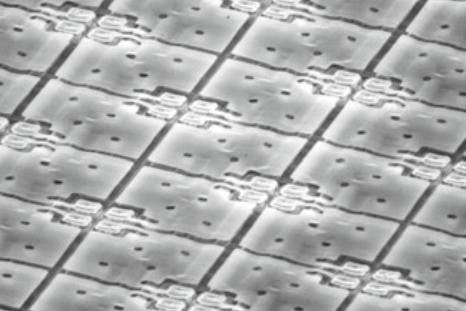
\includegraphics[width=1.0\linewidth, height=5cm]{FPA.png} 
        \caption{}
        \label{FPA}
    \end{subfigure}
    \begin{subfigure}{0.5\textwidth}
        \centering
        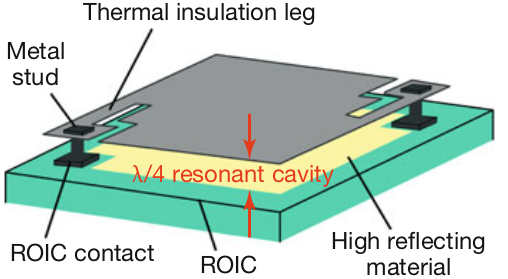
\includegraphics[width=1.0\linewidth, height=5cm]{FPA_pixel.png}
        \caption{}
        \label{FPA_pixel}
    \end{subfigure}

    \caption{(a) Focal point array under electronic microscope. (b) Bolometer with $\lambda /4$ resonant cavity. Image source: Vollmer, Möllmann\cite{thermal_book}}
    \label{FPA_microbolo}
\end{figure}

Absorber material is made either out of metals such as gold, platinum, titanium or more commonly out of semiconductors such as vanadium-oxide (VOx)\cite{thermal_article}.
Important property of absorber materials is that electrical resistance changes proportionally with material's temperature\cite{thermal_book}.
When IR radiation hits absorber material, it is converted into thermal energy, which raises absorber's temperature, thus changing its resistance.
To detect change in resistance, ROIC applies steady-state bias current to absorber material, while measuring voltage over conductive legs\cite{thermal_book}. 

When deciding between different types of thermal cameras we are often comparing them in the terms of cost, size and image resolution.
One important property that also has to be taken into account is temperature sensitivity, also known as noise equivalent temperature difference (NETD).
NETD is measured in \si{\milli\kelvin} and tells us minimum temperature difference that can still be detected by a thermal camera.
In microbolometers NETD is proportional to the thermal conductance of absorber material, among other factors\cite{thermal_book}.
Thermal conductance of bolometers is minimized by enclosing FPA into vacuum chamber, thus excluding thermal convection and conduction due to surrounding gasses.
Only means of heat transfer that remain are radiant heat exchange (highly reflective material below absorber is minimizing its radiative losses) and conductive heat exchange through supportive legs.
NETD also depends on the temperature inside the camera, higher ambient temperatures can raise the internal temperature, thus increasing NETD and noise present in thermal image.
Today's thermopiles can achieve NETD of 100 \si{\milli\kelvin}, microbolometers 45 \si{\milli\kelvin}, while photon detectors can have NETD of 10 \si{\milli\kelvin}.
Although tens of \si{\milli\kelvin} does not seem a lot, we can see on Figure \ref{NETD} what a difference of 20 \si{\milli\kelvin} means for image resolution and noise.
\newline

\begin{figure}[h]
    \begin{subfigure}{0.5\textwidth}
        \centering
        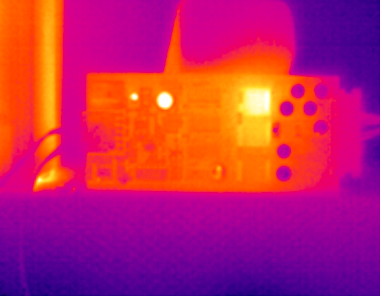
\includegraphics[width=1.0\linewidth, height=5cm]{NETD_60mk.png} 
        \caption{NETD is 60 \si{\milli\kelvin}}
        \label{NETD_60mk}
    \end{subfigure}
    \begin{subfigure}{0.5\textwidth}
        \centering
        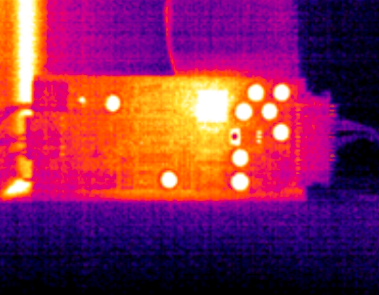
\includegraphics[width=1.0\linewidth, height=5cm]{NETD_80mk.png}
        \caption{NETD is 80 \si{\milli\kelvin}}
        \label{NETD_80mk}
    \end{subfigure}

    \caption{Comparison of images of the same object taken with cameras with different NETD values. Low NETD values are more appropriate for object recognition. Image source: MoviTherm \cite{NETD}}
    \label{NETD}
\end{figure}


\subsection{ Choosing the thermal camera}

Choice of thermal camera was made by Arribada Initiative\cite{thermal_comparison}.
They tested several different thermopiles and microbolometers, while searching for desired properties.
Camera had to be relatively inexpensive and small enough so that it could be integrated into relatively small housing.
Main property that they searched for was that elephants could be easily recognized from thermal images.
That meant that camera needed to have decent resolution and low NETD.
Cameras were tested in Whipsnade Zoo and the Yorkshire Wildlife Park where images of elephants and polar bears could be made.

They tested two thermopile cameras (Heimann 80x64, MELEXIS MLX90640) and two microbolometer cameras (ULIS Micro80 Gen2, FLIR Lepton 2.5).
Although thermopile cameras were cheaper from microbolometer cameras, quality of images they produced was inferior, as can be seen on Figure \ref{thermal_comparison_images}
MELEXIS MLX90640 camera had resolution of 32 x 24 pixels and NETD of 100 \si{\milli\kelvin}, while Heimann camera had resolution of 80 x 64 pixels and NETD of 400 \si{\milli\kelvin}.
\newline

\begin{figure}[h]
    \begin{subfigure}{0.5\textwidth}
        \centering
        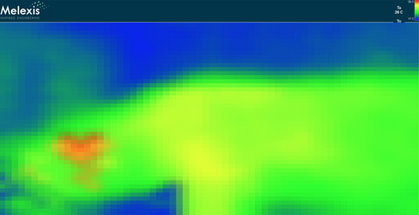
\includegraphics[width=1.0\linewidth, height=5cm]{thermal_comparison_a.png} 
        \label{thermal_comparison_a}
    \end{subfigure}
    \begin{subfigure}{0.5\textwidth}
        \centering
        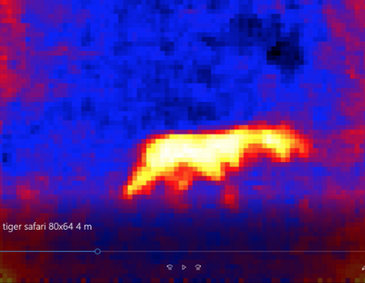
\includegraphics[width=1.0\linewidth, height=5cm]{thermal_comparison_b.png} 
        \label{thermal_comparison_b}
    \end{subfigure}
    \begin{subfigure}{0.5\textwidth}
        \centering
        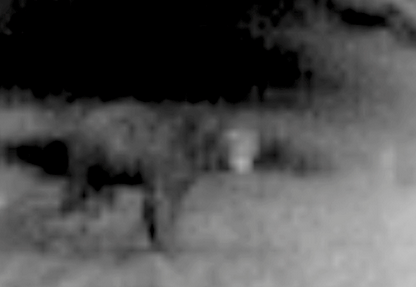
\includegraphics[width=1.0\linewidth, height=5cm]{thermal_comparison_c.png} 
        \label{thermal_comparison_c}
    \end{subfigure}
    \begin{subfigure}{0.5\textwidth}
        \centering
        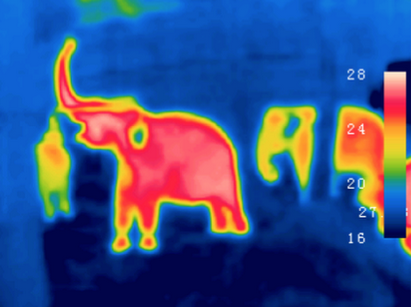
\includegraphics[width=1.0\linewidth, height=5cm]{thermal_comparison_d.png} 
        \label{thermal_comparison_d}
    \end{subfigure}

\caption{Comparison of image quality made by different thermal cameras, MELEXIS MLX90640 (top left), Heimann 80x64 (top right), ULIS Micro80 Gen2 (bottom left) and FLIR Lepton 2.5 (bottom right). Image source: Arribada Initiative \cite{thermal_comparison}}
    \label{thermal_comparison_images}
\end{figure}

It was concluded that images taken by either one of thermopile cameras could not be used for object recognition, merely only if object was present or not\cite{thermal_comparison}.

Microbolometers produced better results.
Both Ulis Micro80 and FLIR Lepton had similar resolution, 80 x 80 and 80 x 60 respectively, but Ulis Micro80 had two times bigger NETD compared to FLIR Lepton camera, 100 \si{\milli\kelvin} and 50 \si{\milli\kelvin}, respectively.
Images produced by FLIR Lepton were much cleaner, so it was chosen as appropriate camera for the task.

It is important to note that FLIR Lepton, as all microbolometers, requires frequent calibration to function properly.
In temperature non-stabilized cameras small temperature drifts can have a major impact on image quality\cite{thermal_book}.
Calibration is done either by internal algorithms of the camera or by exposing the camera to uniform thermal scene.
FLIR Lepton camera comes with a shutter, which acts as a uniform thermal signal and enables regular calibration.
Calibration in FLIR Lepton is by default automatic, triggering at startup and every 3 minutes afterwards or if camera temperature drifts for more than 1.5 \si{\celsius}.


    2.2 Wireless technologies in IOT world
        different technologies, tradeoffs, why do we want lora. 
        2.2.2 LoRa 
            How does it work, what is the ecosystem around it, power consumption, data transmission (compare with some other things) 
    2.3 Neural networks
        What neural networks are, what is their point, forward propagation, back propagation, what kinds of neural networks exist, which ones are interesting for me.
    2.4 TensorFlow
        Describe the framework, what are alternatives, how does it work for you (meaning what programmer doesn't need to care about).
        2.4.1 TensorFlow Lite for microcontollers
            What this is, how is given to developers, describe generic flow from a model to deploying it.
    2.5 Solar panels
        How they work, types, expected power output
    2.6 Battery technologies
        Princips of operation, types, focus on the one you will use, Lipo 
    Above two chapters should be short.

